\chapter{Food and Health}
\begin{chapquote}{Unknown author, \textit{Unknown source of this quote}}
'Role of nutrients, roughage and water in keeping healthy, communicable and non-communicable diseases, and prevention are treatment of diseases.'
\end{chapquote}

\section{Get rolling}
Look at Riya and her freinds. can you tell who has healthy habits? Write Good for healthy habits and Bad for unhealthy ones in the spaces provided.
\begin{itemize}
    \item Riya loves to exercise everyday. \textcolor{green}{Good}
    \item Rohan loves to eat burger and fried food daily. \textcolor{red}{Bad}
    \item Sirman always uses handkerchief while sneezing. \textcolor{green}{Good}
    \item Sia always forgets to cover her mouth while coughing. \textcolor{red}{Bad}
    \item Ruhi loves to eat salad. \textcolor{green}{Good}
\end{itemize}
\section{Learning Objectives}
\begin{itemize}
    \item to recall the role of nutrients in the body
    \item to explain a food pryamid
    \item to discuss different deficiency diseases 
    \item to differentiate between communicable and non-comminucable diseases
\end{itemize}
\section{\textcolor{red}{Nutrients in food}}
We eat food to live and stay healthy. Food provides us with energy and helps in the growth, development and repair of the body. Food also protects us from various diseases. All these functions of food are possible due to the presence of \textcolor{red}{nutrients} in it.\\
\par
There are different types of nutrients, and they all have different 
roles. Let us have a quick recap of nutrients and their roles.
\subsection{\textcolor{orange}{Types of nutrients}}
Nutrients from food, including carbohydrates in items like bread and rice, fat from  sources like nuts and olive oil, are vital for energy and organ protection. Protiens found in dairy products, fish and meat help in growth and body repair. Vitamins and minerals, obtained from fruits and vegetables, support overall health.
\subsection{\textcolor{orange}{Roughage and Water}}
In addition to the essential nutrients, we also require sufficient roughage and water in our diet. Roughage, derived from whole grains and fruits, aids digestion and prevents \textcolor{red}{constipation}. Water is important for temperature regulation, digestion, and transportation of nutrients in the body. Drinking enough water helps us stay hydrated, which is essential for the proper functioning of the body.

\begin{figure}[h]
    \centering
    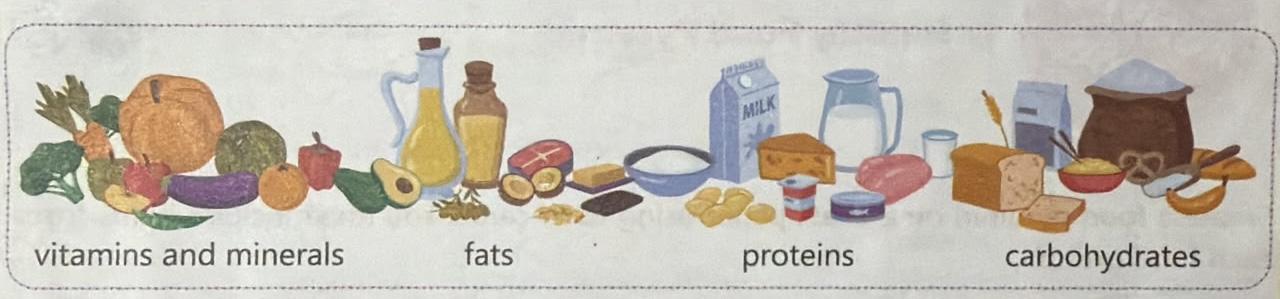
\includegraphics[scale=0.28]{../image/food.jpeg}
    \caption{Nutritious Food}
    \label{fig:nutrious-food}
\end{figure}
\section{\textcolor{red}{Food Pyramid}}
Dietary requirements vary from person to person. Every person has unique factors that influence his or her nutritional needs of a person are age, gender, activity level are health condition. \\
\par

A \textbf{food pyramid} is a visual representation of a balanced diet, showing the different food groups are their recommended quantities for healthy and balanced nutrition.\\
\par
A typical food pyramid consists of several horizontal sections of layers, with each layer representing a different food group.

\begin{figure}[h]
    \centering
    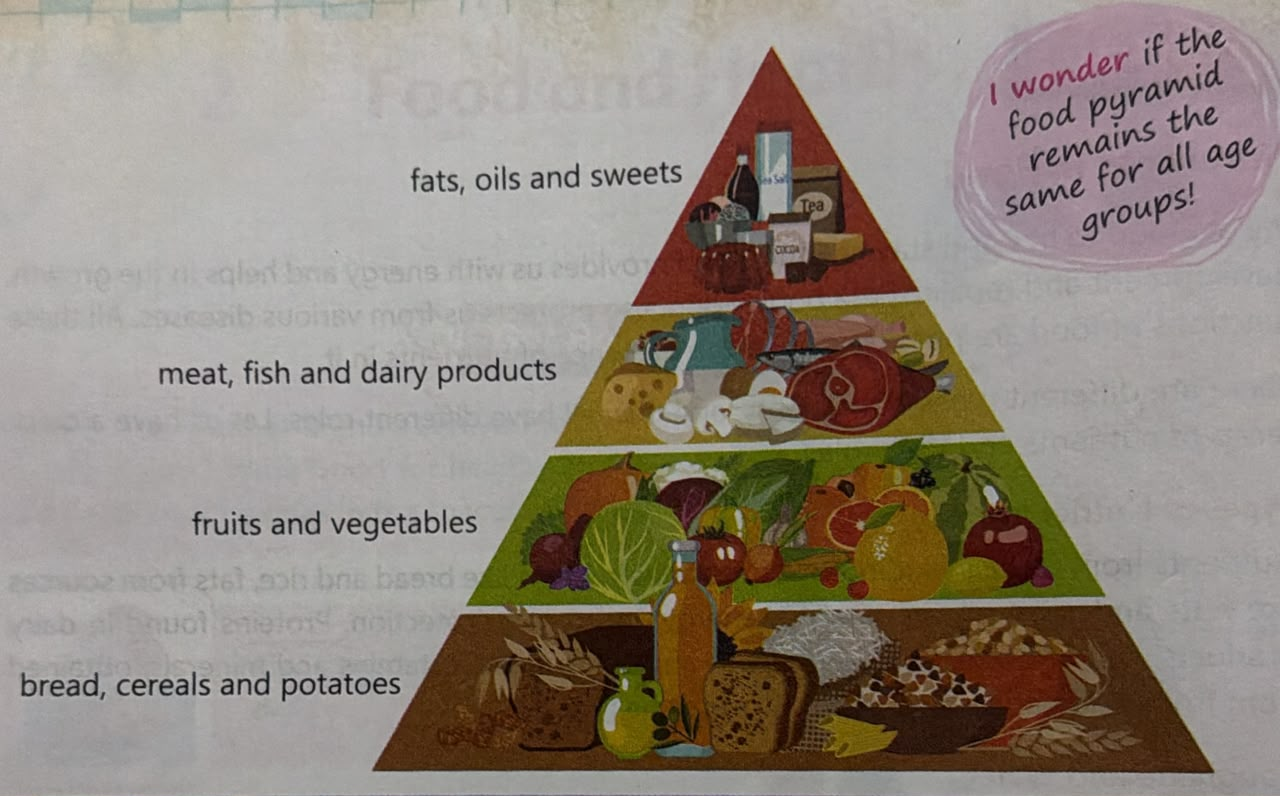
\includegraphics[scale=0.28]{../image/food-pyramid.jpeg}
    \caption{ Food Pyramid}
    \label{fig:food-pyramid}
\end{figure}

Not eating balanced diet or eating a diet that is deficient in one or more nutrients leads to a deficiency of those nutrients in the body. Such a deficiency  of nutrients may lead to \textbf{deficiency diseases.}\\
\par
Let us first understand what diseases are.\\

\section{\textcolor{red}{Diseases}}
When we fall sick, we do not feel like doing anything. This condition when the body is unable to function properly is called a disease. \\
\par
Diseases can be of two types, \textbf{communicable} and \textbf{non-comminucable} depending on whether they can spread one person to another or not.
\section{\textcolor{red}{Non-Communicable Diseases}}
The diseases that do not spread from one person to another are called \textbf{non-communicable diseases.} All deficiency diseases are non-communicable diseases. Let us learn about deficiency diseases.\\ 
\subsection{\textcolor{orange}{Deficiency diseases}}
\textbf{Deficiency diseases} are caused by lack of one more nutrients in the diet. Some common deficiency diseases are their \textcolor{red}{symptom} are summarised in th table below.\\

  \pagebreak
\begin{table}[!h]
    \centering  
\begin{tabular}{|c|c|p{3.7cm}|p{3.4cm}|}
\hline
 \makecell{\textbf{Deficiency} \\ \textbf{disease}} & \makecell{\textbf{Deficiency} \\ \textbf{cause}} & \makecell{\textbf{Common symptoms}} & \makecell{  \textbf{Food to be eaten} \\ \textbf{to avoid deficiency}} \\
 \hline
 anaemia & iron & fatigue, weakness and \textcolor{red}{pale} skin & red meat, poultry, fish, beans, lentils, tofu and spinach\\
 \hline
goitre & iodine & englargement of a gland in the neck region & iodised salt and seafood\\
\hline
tooth decay & calcium & weak and teeth bones & milk, milk products, sprouts, multi-grain cereals and sesame seeds\\
\hline
\makecell{night \\blindness} & vitamin A & poor vision at night & carrots, sweet potatoes, pumpkin, spinach and cod liver oil\\
\hline 
beriberi & vitamin B & extreme tiredness, loss of appetite and loss of muscle function & fish, chicken, eggs, kidney beans and daily products\\
\hline
scurvy & vitamin C & bleeding gums, swelling of joints and impaired wound healing & oranges, lemons, grapefruits, strawberries, kiwi and tomatoes\\
\hline
rickets & vitamin D & weak and brittle bones & egg yolk, milk, mushroom and cod liver oil\\
\hline
marasmus & carbohydrates, proteins, and fats & serve weight loss, fatigue and weakness, and growth impairment and dry and loose skin & rice, wheat, bread, pulses, eggs, milk and fish\\
\hline
kwashiorkor & proteins & scaly skin, thin legs, swollen stomach and ankles & pulses, milk, fish and eggs\\
\hline
\end{tabular}
\caption{Deficiency disease, there cause and food to prevent them}
\end{table}

\section{\textcolor{red}{Overnutrition}}
\textbf{Overnutrition}, or excessive nutrient intake, occurs when a person consumes more nutrients than needed, leading to \textbf{obesity.} Obesity is characterised by excess fat deposits in one's body. If often results from the overconsumption of carbohydrates and fats that are not adequately utilised by the body. This can lead to health issues like high blood pressure and heart diseases.\\
\par
Excessive consumption of junk food, which how is low in nutritional value and high in carbohydrates, sugars, unhealthy fats and salt, in major cause obesity. Examples of junk food include burgers, pizzas, candies, cookies, cakes, pastries, soda, noodles, energy drinks and sweetened juices.
\section{\textcolor{red}{Communicable Diseases}}
\textbf{Communicable diseases} are illensses that can pass from one person to another. These diseases are caused by tiny organisms called \textbf{germs,} which are generally microbes. Microbes are too small to be seen without a microscope. Common types of microbes include bacteria, viruses, protozoa and funji.
\subsection{\textcolor{orange}{Direct Contact}}
Some germs can be transferred through direct physical contact with an infected person. Diseases such as common cold, chickenpox and mealseas spread in this way.
\begin{figure}[h]
    \centering
    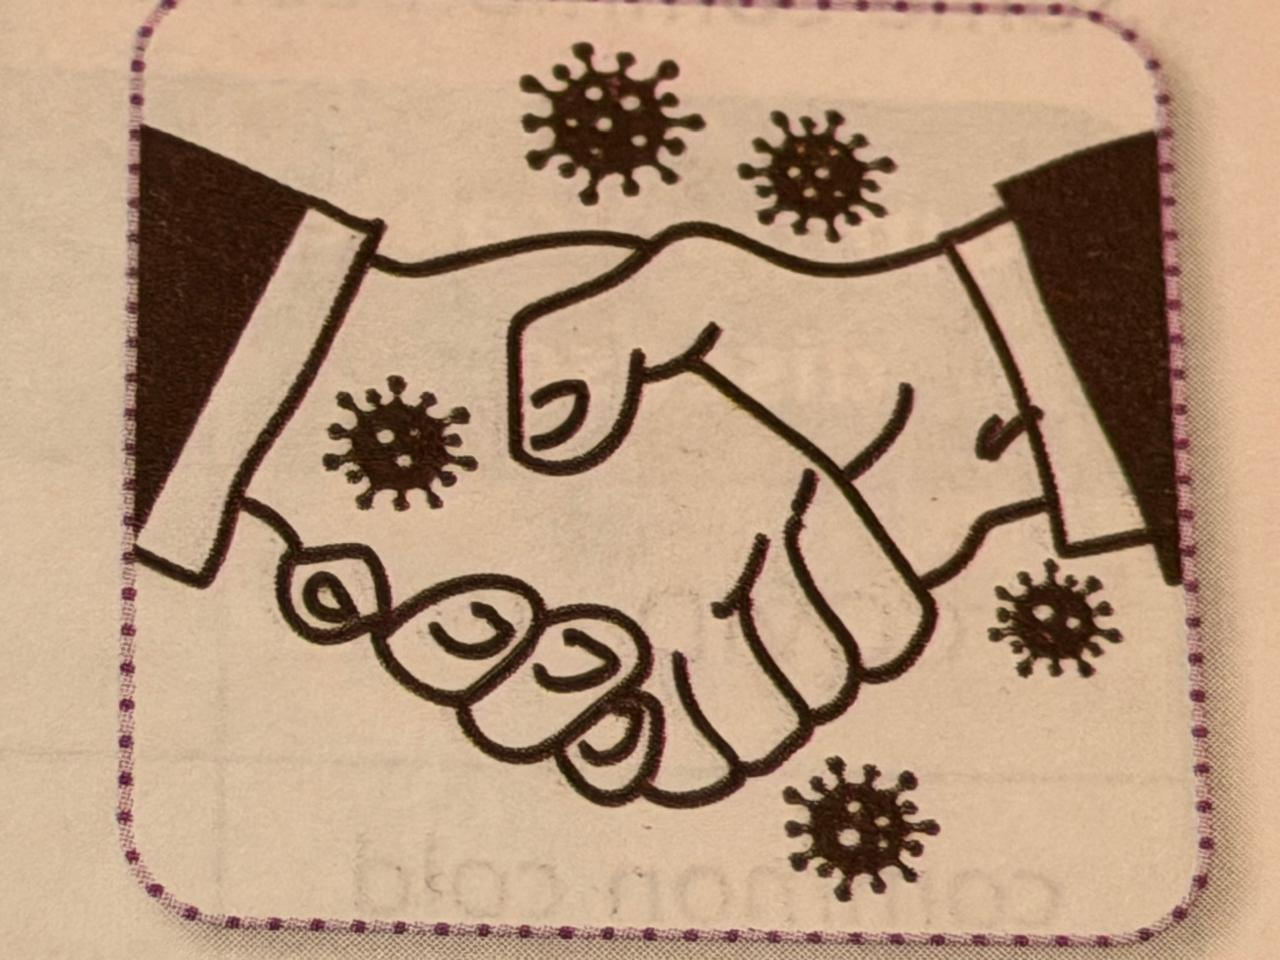
\includegraphics[width=0.5\linewidth]{../image/contact.jpeg}
    \caption{Transfer of disease through handshake}
    \label{fig:contact}
\end{figure}
\subsection{\textcolor{orange}{Indirect Contact}} 
Germs can also be transferred indirectly through objects or surfaces; for example, by touching a doorknob or a surface that has been touched by an infected person and then touching the face. COVID-19 can spread in this manner.
\begin{figure}
    \centering
    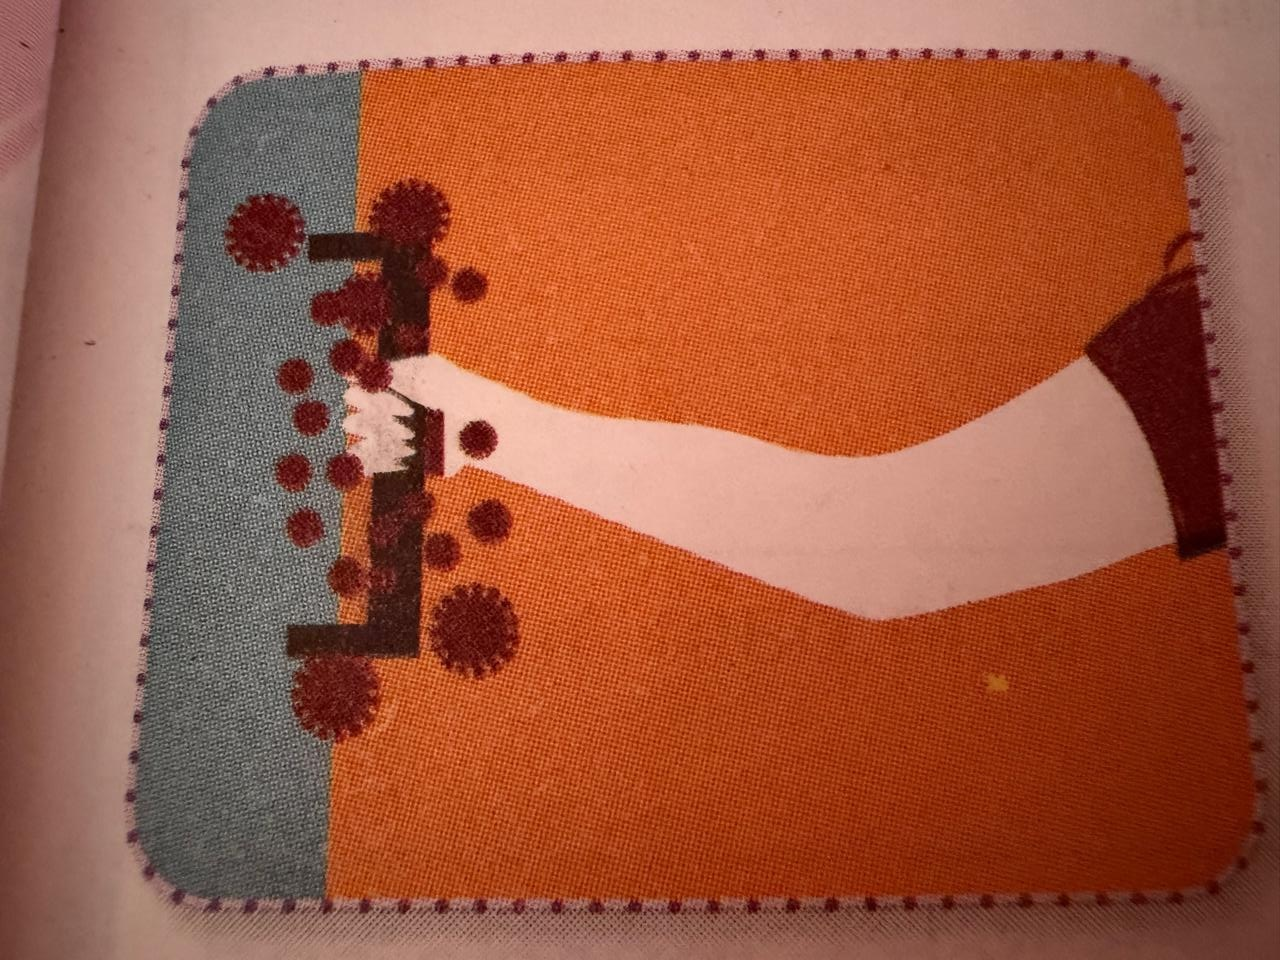
\includegraphics[width=0.5\linewidth]{../image/hand.jpeg}
    \caption{Diseases through Indirect Contact}
    \label{fig:hand}
\end{figure}
\subsection{\textcolor{orange}{Through Air}}
Certain diseases spread when germs are realeased into the air through coughing, sneezing or talking by an infected person. People nearby can inhale these germs, making them infected. Example of such diseases include common cold and whooping cough.
\begin{figure}[!h]
    \centering
    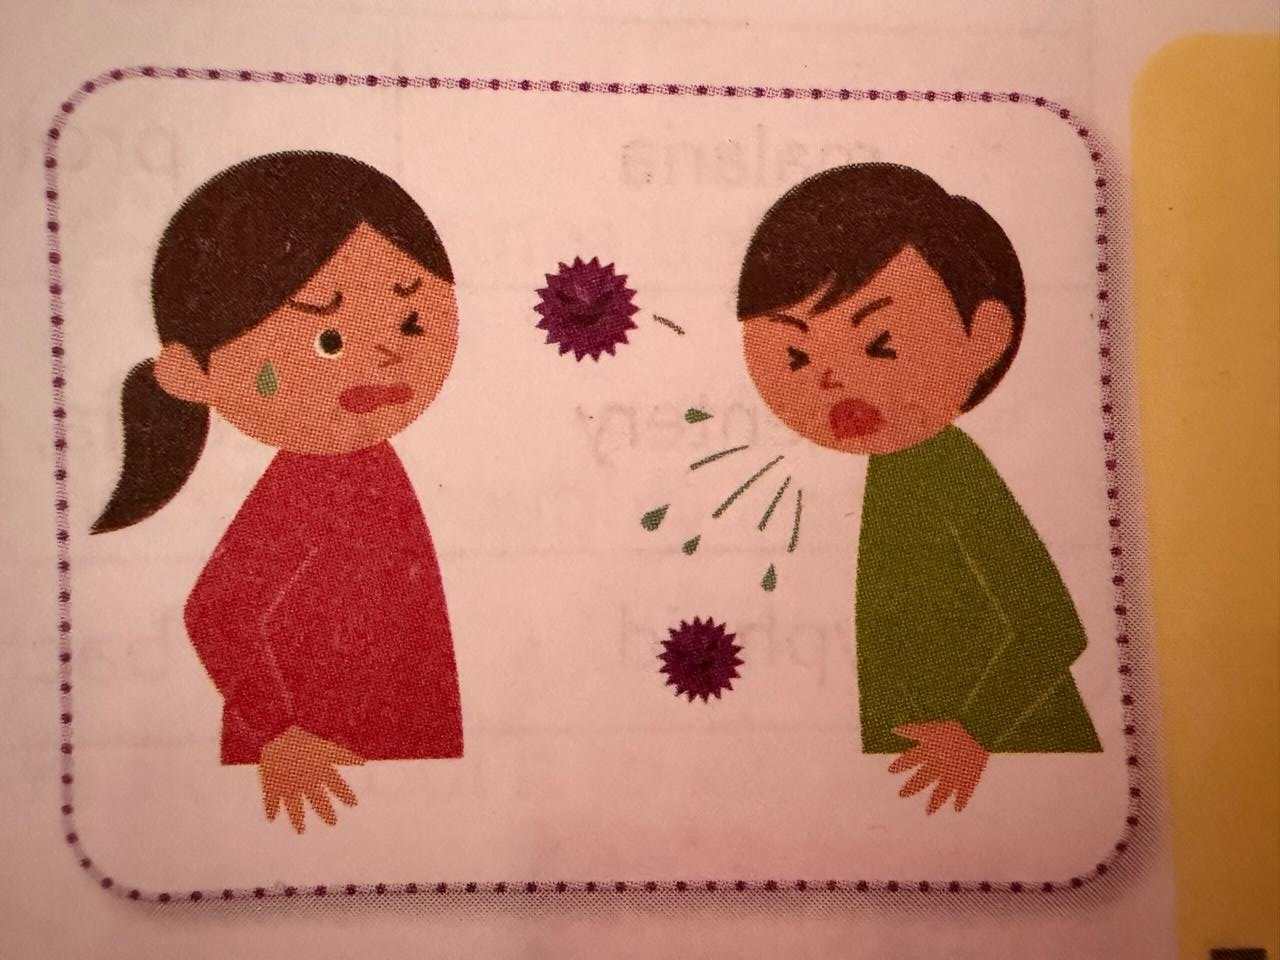
\includegraphics[width=0.5\linewidth]{../image/air.jpeg}
    \caption{Germs with Through Air}
    \label{fig:air}
\end{figure}

\subsection{\textcolor{orange}{Through Water}}
\textcolor{red}{Contaminated} water sources carry germs that cause diseases like cholera and dysentery. When people consume or come into contact with contaminated water, they become infected and acquire such diseases.
\subsection{\textcolor{orange}{Through Food}}
Consuming contaminated food or beverages can lead to the transfer of certain germs, resulting in diseases like diarrhoea and jaundice.

\begin{figure}[!h]
    \centering
    
\includegraphics[width=0.5\linewidth]{../image/contaminated_food.jpeg}
    \caption{Contaminated Through Food}
    \label{fig:cont-food}
\end{figure}

\subsection{\textcolor{orange}{Through Flies and Mosquitoes}}
Certain diseases are transferred by flies and mosquitoes. Flies sit on food, contaminate it and act as a carrier of germs. Mosquitoes suck blood of a person infected with malaria and then bite someone, causing that person to become infected. This way, mosquitoes too act as a carrier of germs.

\begin{figure}[!h]
    \centering
    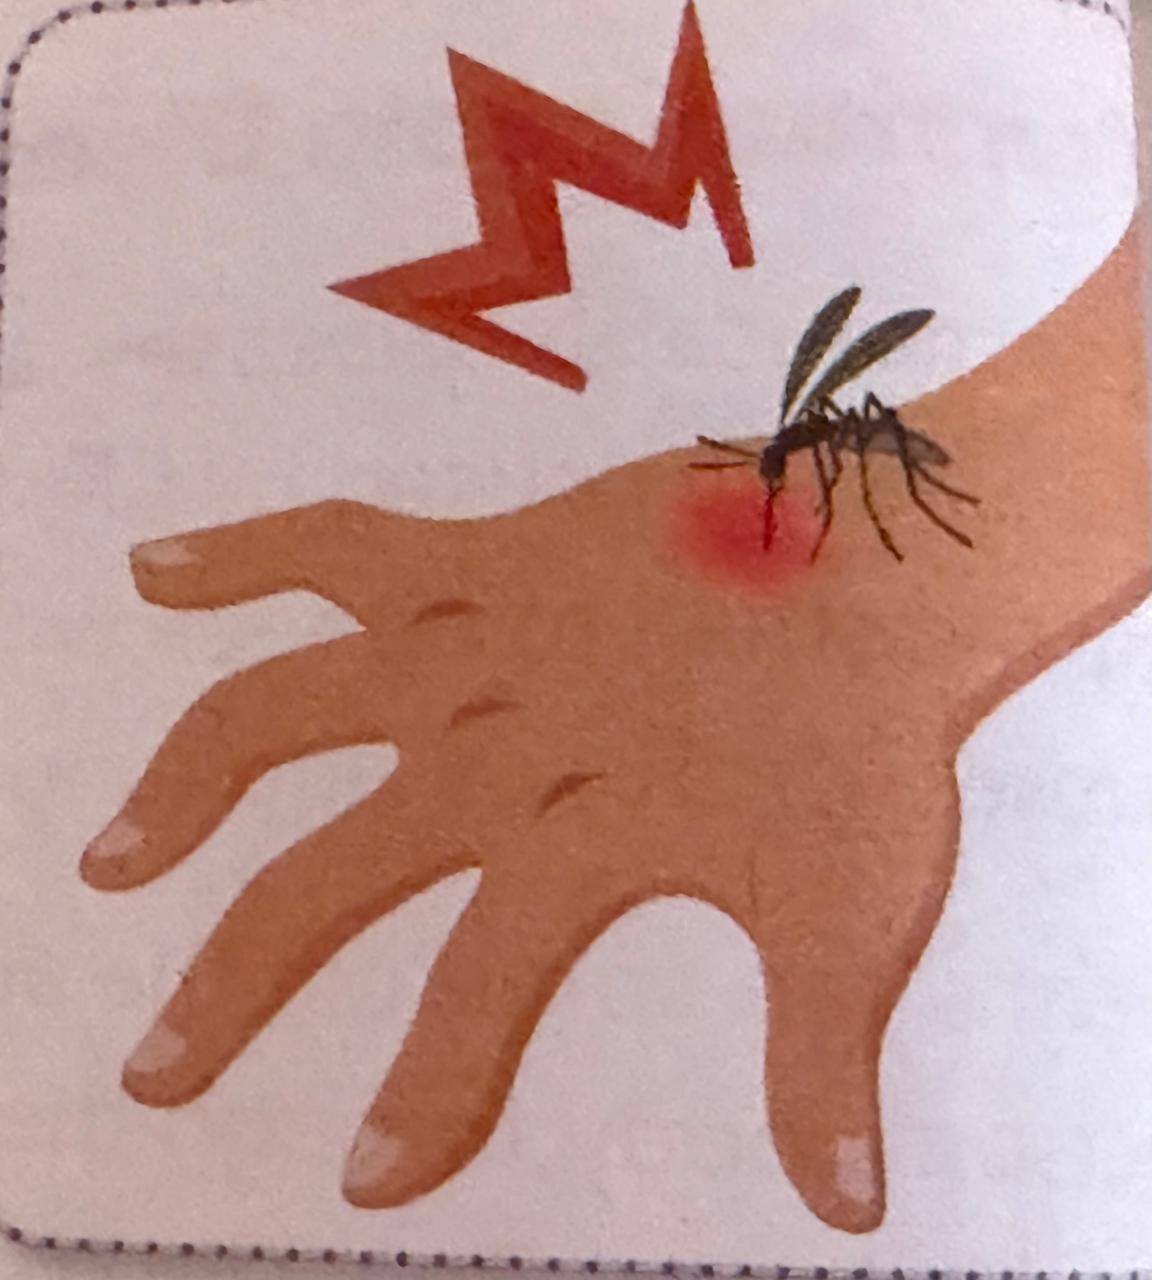
\includegraphics[width=0.5\linewidth]{../image/mosquito_bite.jpeg}
    \caption{Diseases through flies and mosquitoes}
    \label{fig:mosq}
\end{figure}

Some common communicable diseases are summarised in the table below.
\begin{table}[!h]
\centering
    
    \begin{tabular}{|c|c|c|}
    \hline
Communicable diseases & \textbf{Cause} & \textbf{Symptoms} \\
\hline
COVID-19 & virus & cough, cold, fever, sore throat and shortness of breath\\
\hline
common cold & virus & cough, cold and sore throat\\
\hline
measles & virus & runny nose, sore throat, white sports inside the mouth and fever\\
\hline
chickenpox & virus & rashes, fever and body pain\\
\hline
dengue & virus & high fever, rashes, joint and muscle pain and tiredness\\
\hline
malaria & protozoa & fever, chills, headache, stomach ache, muscle and joint pain\\
\hline
dysentery & bacteria, protozoa & diarrhoea, stomach ache, fever, dehydration, and vomiting\\
\hline
typhoid & bacteria & fever, tierdness, loss of appetite and stomach ache\\
\hline
    \end{tabular}
    \caption{Tables of Communicable Diseases}
    \label{tab:communicable-disease}
\end{table}

\section{\textcolor{red}{Prevention of Communicable Diseases}}
Preventing the spread of communicable diseases involves simple measures:
\subsection{\textcolor{orange}{Personal and Hygiene and Care}}
1. Frequent handwashing: Wash hands with soap and water to remove germs, reducing infection risk.\\
2. Avoid handshakes: Minimise and physical contact.\\
3. Maintain person cleanliness: Take daily baths, wear clean clothes, cover the mouth and the nose when coughing or sneezing.\\
4. Exercise and rest: Proper exercise and rest keep us fit and healthy.\\
\begin{figure}
    \centering
    
\includegraphics[width=0.5\linewidth]{../image/exersice .jpeg}
    \caption{Practice excersice every day}
    \label{fig:exercise}
\end{figure}
\subsection{\textcolor{orange}{Environmental Hygiene}}
1. Prevent stagnant water: Prevent water accumulation, as mosquitoes breed in stagnant water.\\
2. Proper waste disposal: Use dustbins, cover kitchen waste and keep windows open to let in fresh air and sunlight.\\
3. Mosquito control: Use nets and coils to repel or kill mosquitoes.
\subsection{\textcolor{orange}{Safe Water and food particles}}
1. Ensure clean water: Purify tap water using RO or boil it for 10 - 15 minutes before consumption. \\
2. Eat fresh and clean food: Wash vegetables and fruits, cook food thoroughly and avoid eating food exposed to flies.\\
3. Pasteurize milk: Boil milk at a high temperature, and they rapidly cool it to kill the germs present in it.
\subsection{\textcolor{orange}{Vaccination}} 
Get vaccinated: Vaccination is crucial to prevent the spread of communicable diseases.\\
\par
A \textbf{vaccine} contains dead or weakened germs that cause a particular disease. This helps in developing immunity against that disease. This process of administering a vaccine is called \textbf{vaccination.}\\
\par
Vaccine, administered through injection or orally, provide immunity against diseases like polio, measlses, typhoid and COVID - 19.\\
\begin{figure}
    \centering
    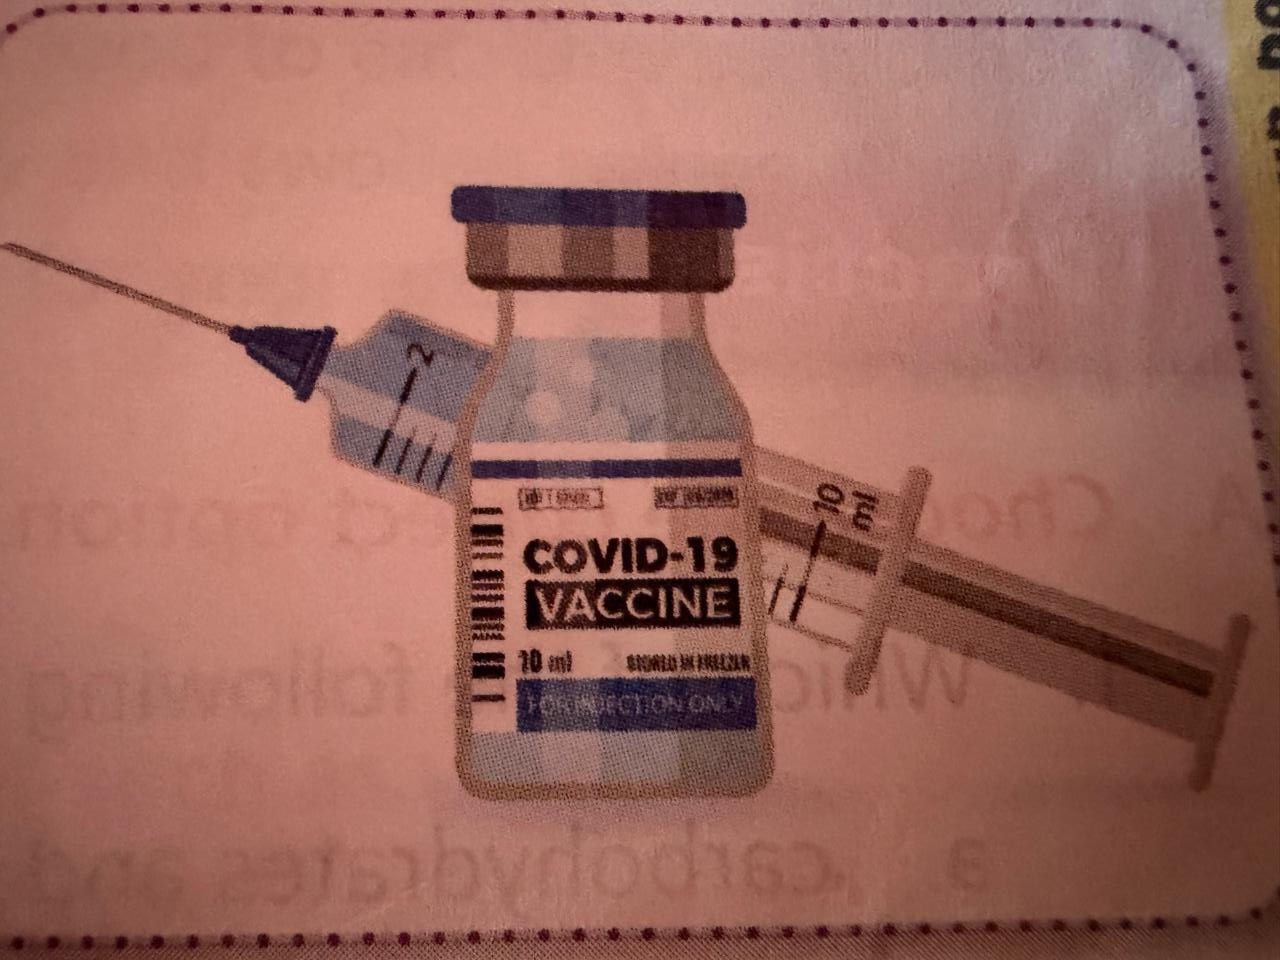
\includegraphics[width=0.5\linewidth]{image/COVID-19.injection.jpeg}
    \caption{COVID - 19 injection}
    \label{fig:vaccine}
\end{figure}
\par
\textcolor{red}{I wonder} of vaccines are made from microbes, why they don't cause diseases!
\begin{itemize}
    \item \textbf{Nutrients} are vital for proper growth and development of the body.\\
    \item Carbohydrates, fats, proteins, vitamins and minerals are the essential nutrients in food.\\
    \item Apart from essential nutrients, our body also needs roughage and water.\\
    \item A \textbf{food pyramid} is the visual representation of all the essential nutrients in right quantities to support good health and well-being.\\
    \item Diseases are of two types, communicable and non-communicable, depending on whether they can spread from one person to another or not.\\
    \item Deficiency diseases are non-communicable and occur due to an insufficient intake of specific vital nutrients.
    \item The diseases that can spread from one person to another are called \textbf{communicable diseases.} These diseases are spread by tiny organisms called \textbf{germs.}
\end{itemize}
